
 Let 
    \begin{align}
        \vec{A}=\myvec{2\\-4\\-5}, \vec{B}=\myvec{1\\-2\\-3}
    \end{align}
    be the adjacent sides of the parallelogram. Let $\vec{D}$ be the diagonal of the parallelogram. Then,
    \begin{align}
        \vec{D}&=\vec{A}+\vec{B}\\
&=\myvec{3\\-6\\-8}
    \end{align}
   \begin{align}
       \norm{\vec{D}}=\sqrt{(3)^2+(-6)^2+(-8)^2}=\sqrt{109}
   \end{align}
   Let $\vec{U}$ be the unit vector of $\vec{D}$ which can be found as follows:
   \begin{align}
       \vec{U}=\frac{\vec{D}}{\norm{\vec{D}}}
   \end{align}
   Solving the above equation gives the unit vector $\vec{U}$ which is parallel to the diagonal $\vec{D}$.\\
   \begin{align}\therefore
       \boxed
       {\vec{U}=\frac{1}{\sqrt{109}}\myvec{3\\-6\\-8}}
   \end{align}
  %   \begin{align}
%        \norm{\vec{A}\times\vec{B}}
%    \end{align}
%    where
   \begin{align}
  \because     \vec{A}\times\vec{B} &=\myvec{0&-A_3&A_2\\A_3&0&-A_1\\-A_2&A_1&0}\myvec{B_1\\B_2\\B3}\\
       &=\myvec{0&5&-4\\-5&0&-2\\4&2&0}\myvec{1\\-2\\-3}=\myvec{2\\1\\0},
       \\
       \norm{\vec{A}\times\vec{B}}&=\sqrt{(-2)^2+(1)^2+(0)^2}\\
       &=\sqrt{5}
\end{align}
which is the desired area.  
% \centering
% 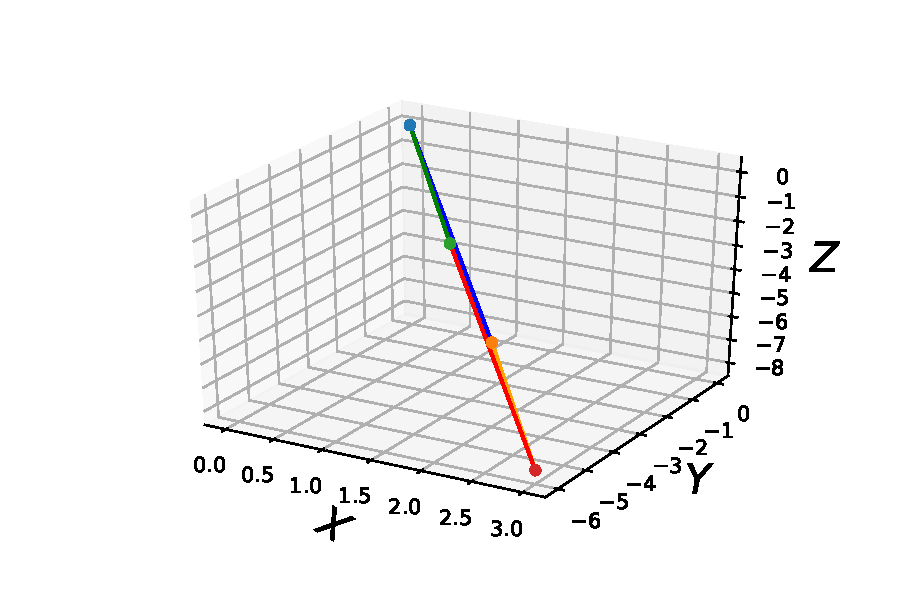
\includegraphics[width=\columnwidth]{solutions/july/1/Figures/parallelogram.pdf}
% \caption{}
% \label{Fig 1.2}
% \end{figure}

